% mainfile: ../../../../master.tex
\subsection{DNA and RNA quantification with Qubit\texttrademark~ assays}
% The part of the label after the colon must match the file name. Otherwise,
% conditional compilation based on task labels does NOT work.
\label{task:20180202_cj0}
\tags{dna,rna,lab,qnt}
\authors{cj}
%\files{}
%\persons{}

\sidenote{Qubit\texttrademark~ dsDNA BR Assay Kit (\texttt{REF \#Q32850}) opened by Elísabet on 20170815; \texttt{LOT: 1835789}.}
\begin{figure}[H] % position of the figure 
    \centering
    \caption{Illustration for the Qubit\texttrademark~ DNA BR assay to quantify DNA extracted with the MasterPure\texttrademark~ kit}
    \label{fig:20180202_DNA_Qubit_assay}
    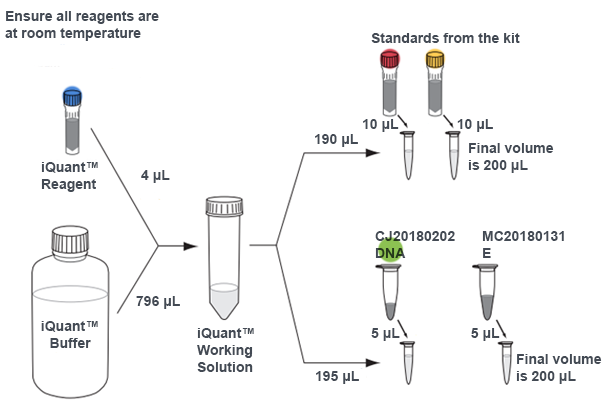
\includegraphics[width=\textwidth]{graphics/schemas/20180202_DNA_Qubit_assay.png}
\end{figure}

\begin{table}[htbp]
\caption{Total DNA quantities in samples measured with Qubit RNA HS Assay Kit}
\label{tab:20180202_nuc_acid_qnt_dna}
\centering
\begin{tabular}{l l r r r r}
\toprule
 & Sample ID & \textmu g/mL & $V_f$ (mL) & m (\textmu g) & m (ng) \\ \midrule
DNA & \texttt{CJ20180202\_DNA} & 3.11 & 0.043 & 0.133 & 133.73 \\
DNA & \texttt{MC20180131\_E} & 3.54 & 0.043 & 0.152 & 152.22 \\
\bottomrule
\end{tabular}
\end{table}

\subsubsection{RNA}

\begin{table}[htbp]
\caption{Total RNA quantities in samples measured with Qubit RNA HS Assay Kit}
\label{tab:20180202_nuc_acid_qnt_rna}
\centering
\begin{tabular}{l l r r r r}
\toprule
 & Sample ID & \textmu g/mL & $V_f$ (mL) & m (\textmu g) & m (ng) \\ \midrule
RNA & \texttt{CJ20180202\_RNA} & 8.65 & 0.043 & 0.371 & 371.95 \\
\bottomrule
\end{tabular}
\end{table}